\documentclass{article}

\usepackage{graphicx}
\usepackage{tikz}
\usepackage{tikzsymbols}
\usetikzlibrary{calc,patterns,shapes.geometric}
\pagestyle{empty}
\usepackage[margin=0pt]{geometry}
\geometry{papersize={14in,12in}}

\def\centerarc[#1](#2)(#3:#4:#5){\draw[#1] ($(#2)+({#5*cos(#3)},{#5*sin(#3)})$) arc (#3:#4:#5);}

\begin{document}
	\begin{figure}
		\centering
		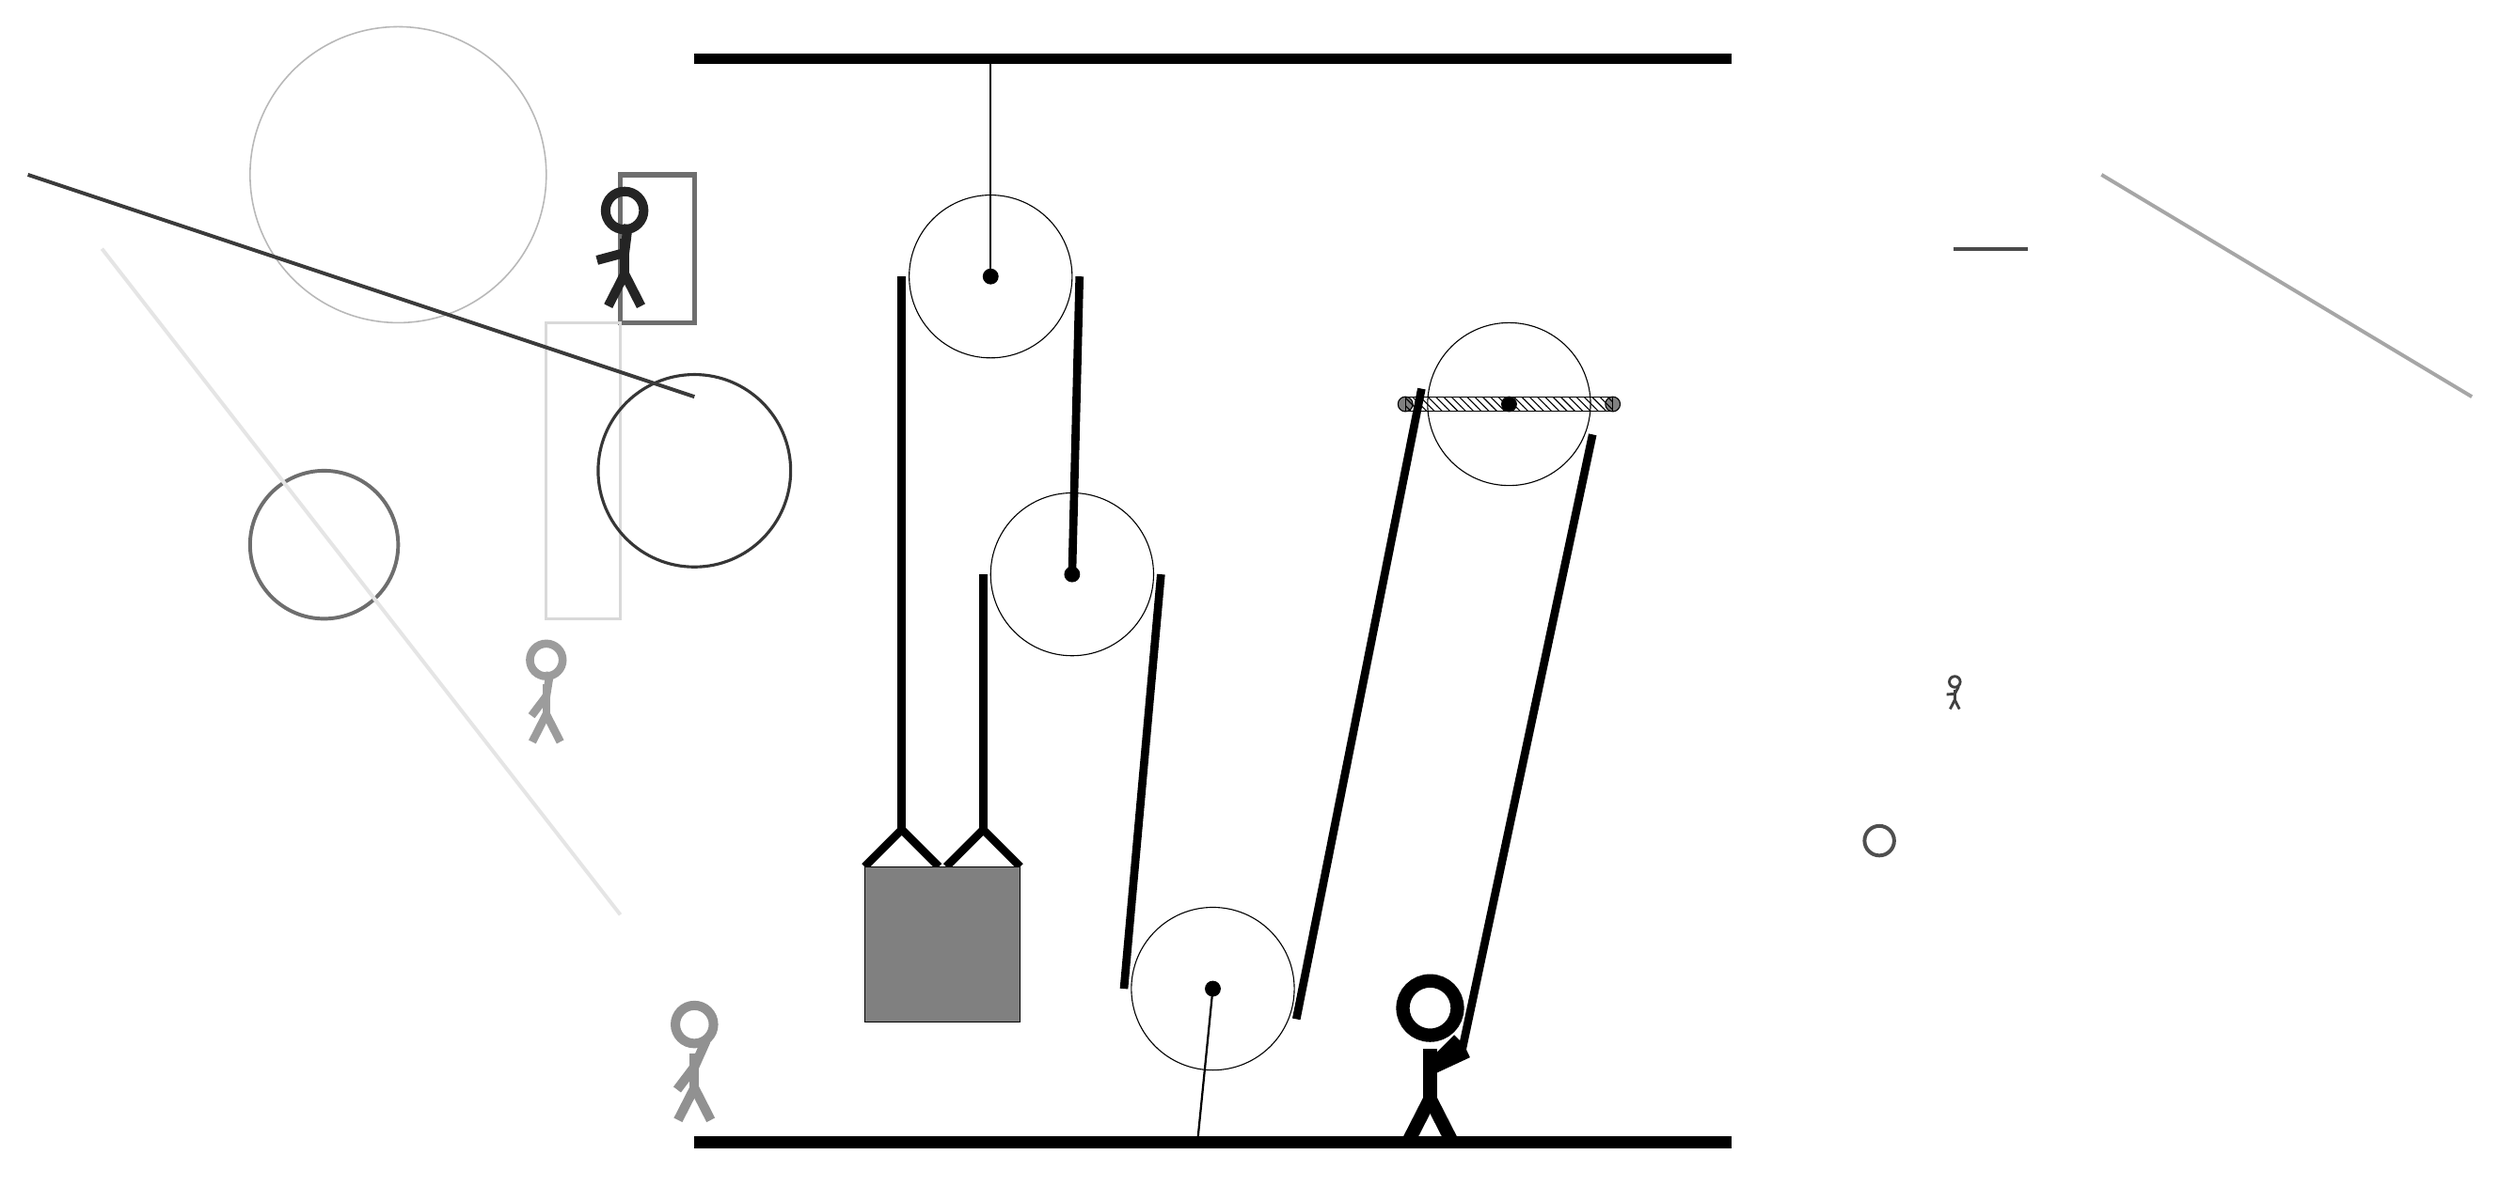
\begin{tikzpicture}
			%%%%% START %%%%%
			
			\draw[fill=black] (-2, 11.5) rectangle (12, 11.625);
			
			\draw (2, 8.625) circle (1.1);
			\draw[fill=black] (2, 8.625) circle (0.1);
			\draw[thick] (2, 8.625) -- (2, 11.5);
			
			\draw (3.1, 4.6) circle (1.1);
			\draw[fill=black] (3.1, 4.6) circle (0.1);
			
			\draw (5, -1) circle (1.1);
			\draw[fill=black] (5, -1) circle (0.1);
			\draw[thick] (5, -1) -- (4.8, -3);
			
			\draw (9, 6.9) circle (1.1);
			\draw[fill=black] (9, 6.9) circle (0.1);
			\draw[fill=black!50] (7.6, 6.9) circle (0.1);
			\draw[fill=black!50] (10.4, 6.9) circle (0.1);
			\draw[pattern=north west lines, pattern color=black] (7.6, 7.0) rectangle (10.4, 6.8);
			
			\draw [line width=0.5mm, color=black!69](14, 1) circle (0.2);
			
			\draw[line width=0.5mm, color=black!35](17, 10) -- (22, 7);
			\draw [line width=0.2mm, color=black!28](-6, 10) circle (2.0);
			\draw[line width=0.7mm, color=black!57] (-3, 8) rectangle (-2, 10);
			\draw[line width=0.5mm, color=black!71](15, 9) -- (16, 9);
			
			\draw [line width=0.5mm, color=black!57](-7, 5) circle (1.0);
			\draw[line width=0.4mm, color=black!15] (-3, 4) rectangle (-4, 8);
			
			\node[line width=0.6mm, color=black!43] at (-2, -2) {\Strichmaxerl[7][53][66]};
			\draw [line width=0.4mm, color=black!79](-2, 6) circle (1.3);
			
			\node[line width=0.6mm, color=black!86] at (-3, 9) {\Strichmaxerl[7][15][83]};
			\draw[line width=0.5mm, color=black!77](-2, 7) -- (-11, 10);
			\node[line width=0.3mm, color=black!39] at (-4, 3) {\Strichmaxerl[6][53][81]};
			\node[line width=0.7mm, color=black!75] at (15, 3) {\Strichmaxerl[2][4][62]};
			
			\draw[line width=0.5mm, color=black!10](-3, 0) -- (-10, 9);
			
			\draw[line width = 1.1mm]  (0.3, 0.65) -- (0.8, 1.15) -- (1.3, 0.65);
			\draw[line width = 1.1mm]  (1.4, 0.65) -- (1.9, 1.15) -- (2.4, 0.65);
			\draw[fill=black!50] (0.3, 0.65) rectangle (2.4, -1.45);
			
			\draw[line width = 1.1mm] (0.8, 8.625) -- (0.8, 1.15);
			\centerarc[line width = 1.1mm](2, 8.625)(0:180:1.2000000000000002);
			\draw[line width = 1.1mm] (3.2, 8.625) -- (3.1, 4.6);
			\draw[line width = 1.1mm] (1.9, 4.6) -- (1.9, 1.15);
			\centerarc[line width = 1.1mm](3.1, 4.6)(0:180:1.2000000000000002);
			\draw[line width = 1.1mm] (4.3, 4.6) -- (3.8, -1);
			\centerarc[line width = 1.1mm](5, -1)(180:340:1.2000000000000002);
			\draw[line width=1.1mm](6.1276, -1.4104) -- (7.8182, 7.1083);
			\centerarc[line width = 1.1mm](9, 6.9)(-20:170:1.2000000000000002);
			\draw[line width=1.1mm](10.1276, 6.4896) --  (8.35, -1.9);
			
			\node at (8, -2) {\Strichmaxerl[10][225][25]};
			
			\draw[fill=black] (-2, -3) rectangle (12, -3.15);
			
			%%%%% END %%%%%
		\end{tikzpicture}
	\end{figure}	
\end{document}